\chapter{Vectorized Backtesting}


Backtesting is the process of testing a trading strategy using historical data, allowing traders to evaluate and refine their
strategies before implementing them in live markets.
In this project, the implemented backtester provides vectorized backtesting for both technical indicator-based strategies
and machine learning-based strategies.
Vectorization, a form of array programming, allows operations typically done on scalars to be extended to multidimensional arrays.
In Python's data ecosystem, \textit{pandas}, with its \textit{DataFrame} class, deeply integrates with \textit{NumPy}, benefiting from
its vectorization principles.
It facilitates compact code, faster execution compared to conventional Python loops, and efficient handling of time series data.
This is particularly useful in financial algorithm implementations, especially vectorized backtesting.

\section{Input Data}


All the data used in this project is downloaded using the \texttt{data\_retriever} module, which establishes a connection with the Binance server
 and downloads data for defined crypto symbols (a crypto symbol represents a specific cryptocurrency,
like BTC for Bitcoin or ETH for Ethereum) over a specified time span and interval.
The downloaded data is stored in the \texttt{historical\_data} directory. Each symbol has its own directory, where the corresponding data is
saved in a \texttt{.csv.parquet} format.
Data is downloaded at a one-minute frequency but can be downsampled to longer intervals, such as 1 hour or 1 day.

The \texttt{load\_data.py} module facilitates loading the historical data of a symbol from its \texttt{.csv} file for use in backtesting strategies.

\begin{figure}[h]
\dirtree{%
.1 backtester.
.2 historical\_data.
.3 BTCUSDT.
.3 ETHUSDT.
.3 \ldots.
.2 \ldots.
.2 utilities.
.3 data\_utils.
.4 data\_loader.py.
.4 data\_manager.py.
.4 data\_retriever.py.
}

\caption{Data-centric modules and folders.}\label{fig:inputdata}
\end{figure}

\section{Technical Indicator-based Strategies}

Technical indicators are mathematical calculations based on historical price, volume, or open interest information that aim to predict future price movements.
Commonly used in technical analysis, these indicators provide insight into the market's direction, strength, momentum, and volatility.
Currently, the backtester supports technical indicators such as BB, EMA, RSI, MACD, SMA, and SO. However, it's designed to easily
accommodate and backtest additional technical indicators as needed.
The backtesting architecture, including relevant classes and components for technical indicator-based strategies, is illustrated in UML diagram \ref{fig:tech_indicator_arch}.

Technical indicators are mathematical calculations based on historical price, volume, or open interest information that aim to predict future price movements.
Commonly used in technical analysis, these indicators provide insight into the market's direction, strength, momentum, and volatility.
\noindent

\begin{figure}[ht!]
\centering
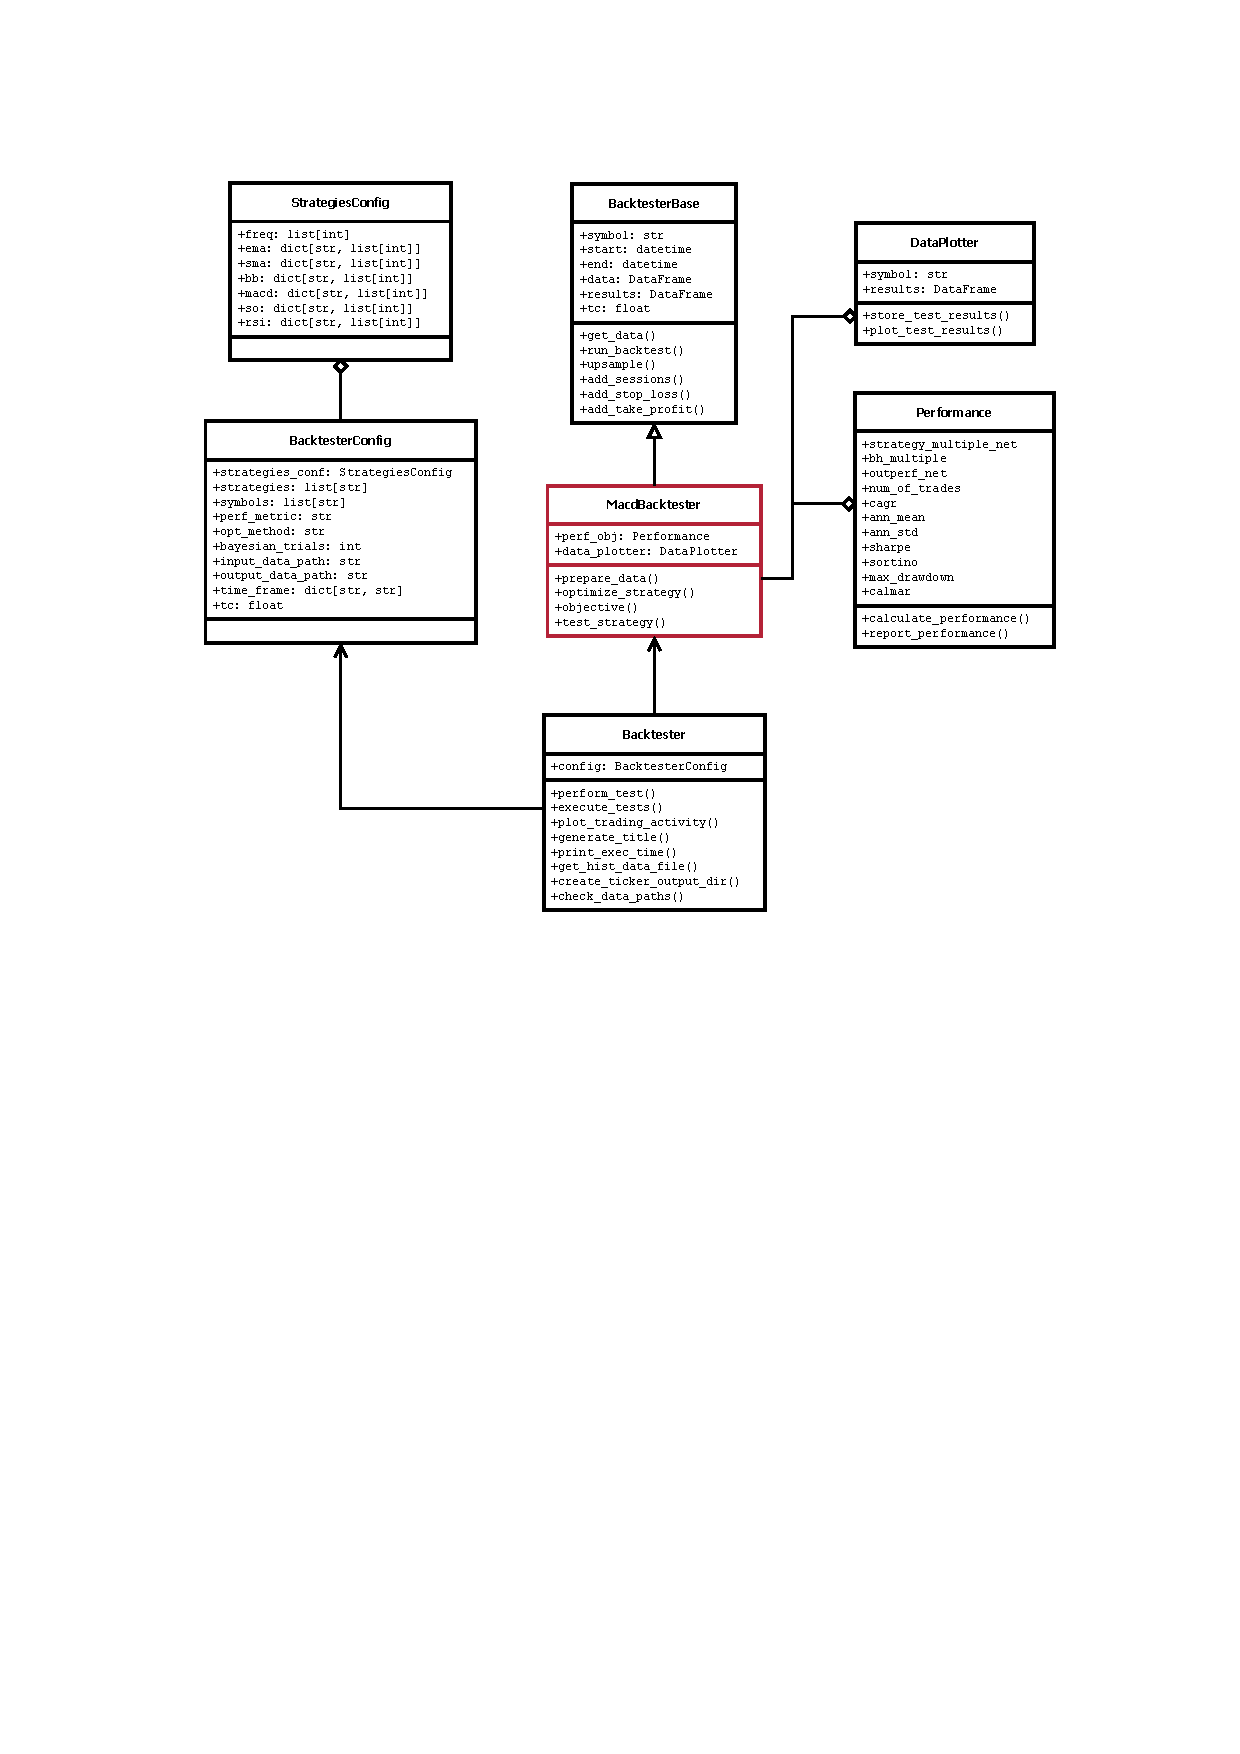
\includegraphics[page=1, trim=30mm 135mm 0 25mm, width=1.1\textwidth, clip]{./uml/backtester_uml.pdf}
\caption{Technical indicator based backtesting architecture.}
\label{fig:tech_indicator_arch}
\end{figure}

\noindent
Technical indicators are mathematical calculations based on historical price, volume, or open interest information that aim to predict future price movements.
Commonly used in technical analysis, these indicators provide insight into the market's direction, strength, momentum, and volatility.

The cornerstone of this framework lies in its automated, vectorized backtesting, which furnishes a remarkably efficient backtesting utility.
The framework incorporates two distinct backtesting variations: one for machine learning-based models and another for technical indicator-based models.
A notable feature of the framework is its extensibility; new testing algorithms can be seamlessly incorporated and configured.
For integration, each new algorithm should inherit from the \texttt{BacktesterBase} class, located in the \texttt{backtester\_base.py} module.
Furthermore, they must implement the methods: \texttt{prepare\_data}, \texttt{optimize\_strategy}, \texttt{objective()}, and \texttt{test\_strategy()}.

Figure \ref{fig:tech_indicator_arch} delves into the architecture of the technical indicator-based backtesting component within the framework.
Notably, the UML class (delineated in red) titled \texttt{MacdBacktester} is a descendant of the \texttt{BacktesterBase} class.
This base class equips all models with essential methods such as \texttt{get\_data}, \texttt{run\_backtest}, \texttt{add\_stop\_loss}, and \texttt{add\_take\_profit}, to name a few.
Additional classes, namely \texttt{DataPlotter} and \texttt{Performance}, are harnessed to compute and graphically represent performance metrics for each test.

A pivotal aspect of this framework is the adaptability of each algorithm's parameters.
Users have the flexibility to configure the parameter spaces via the JSON file named \texttt{backtesterconfig}.
This configuration is subsequently ingested and validated through \texttt{pydantic}.
For optimization, users can employ either the grid search method or the Bayesian method.
While grid search explores all possible combinations in the parameter space, the Bayesian approach uses probability distributions to improve the search.
Given the configuration of parameter spaces for each algorithm, numerous combinations---potentially tens of thousands---can be tested for each symbol.
The performance results for all these combinations are consolidated into a single CSV file, facilitating subsequent analysis.

Consider the snapshot below, extracted from a more intricate configuration, as a case in point:
\begin{verbatim}
{
    "opt_method": "bayesian",
    "bayesian_trials": 1500,
    "time_frame": {
      "start_date": "",
      "end_date": "2022-12-31 23:59:00"
    },
    "symbols": ["XRPUSDT", "LTCUSDT", "TRXUSDT"],
    "strategies_config":
    {
      "freq" : [5, 125, 5],

      "ema": {
          "ema_s": [6, 60, 4],
          "ema_l": [10, 200, 5]
      }
    }
}
\end{verbatim}



Furthermore, individual backtesting results for each symbol and strategy can be visualized, as depicted in fig.~\ref{fig:backtest_results}.
This figure showcases the performance results of the optimized strategy juxtaposed against the buy-and-hold strategy.
As an illustrative example, the EMA strategy for LTCUSDT is spotlighted. All pertinent parameters are illustrated above the primary plot.
Testing was executed on historical data spanning from 2021-01-01 to 2021-12-31.
The secondary plot, detailing close prices, accentuates the drastic price fluctuations during this period.
 Impressively, the algorithm managed to surpass the buy-and-hold strategy, achieving an outperformance of 0.953 (which can be construed as a 95\% enhancement).

\begin{table}[ht!]
    \centering
    \begin{tabular}{l}
        \texttt{LTCUSDT | EMA : (plot\_all = True , freq = 125 , ema\_s\_val = 50 , ema\_l\_val = 200 )} \\
        \texttt{Strategy Multiple = 2.065 , Buy/Hold Multiple = 1.09 ,} \\
        \texttt{Net Out-/Under Perf = 0.953 , Num Trades = 14} \\
    \end{tabular}
\end{table}


\begin{figure}
\centering
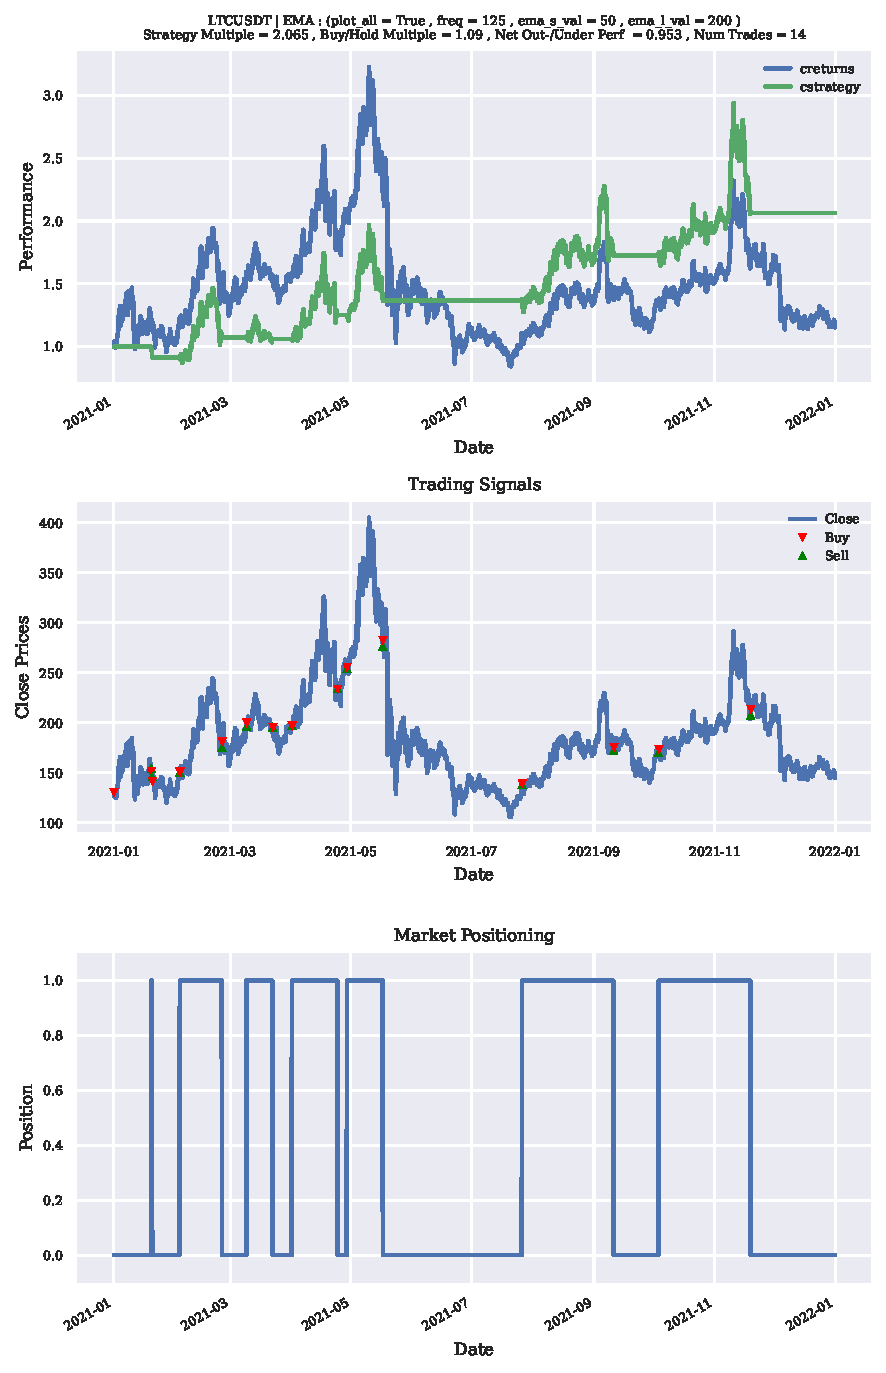
\includegraphics[page=1, trim=0mm 0mm 0 0mm, width=1\textwidth, clip]{./uml/backtesting_results.pdf}
\caption{Results of Backtesting of MACD Stragegy of XRPUSDT.}
\label{fig:backtest_results}
\end{figure}

Furthermore, individual backtesting results for each symbol and strategy can be visualized, as depicted in fig.~\ref{fig:backtest_results}.
This figure showcases the performance results of the optimized strategy juxtaposed against the buy-and-hold strategy.
As an illustrative example, the EMA strategy for LTCUSDT is spotlighted. All pertinent parameters are illustrated above the primary plot.
Testing was executed on historical data spanning from 2021-01-01 to 2021-12-31.
The secondary plot, detailing close prices, accentuates the drastic price fluctuations during this period.
 Impressively, the algorithm managed to surpass the buy-and-hold strategy, achieving an outperformance of 0.953 (which can be construed as a 95\% enhancement).
% trim={<left> <lower> <right> <upper>}
%\vspace{-2cm}

\begin{figure}[h]
\centering
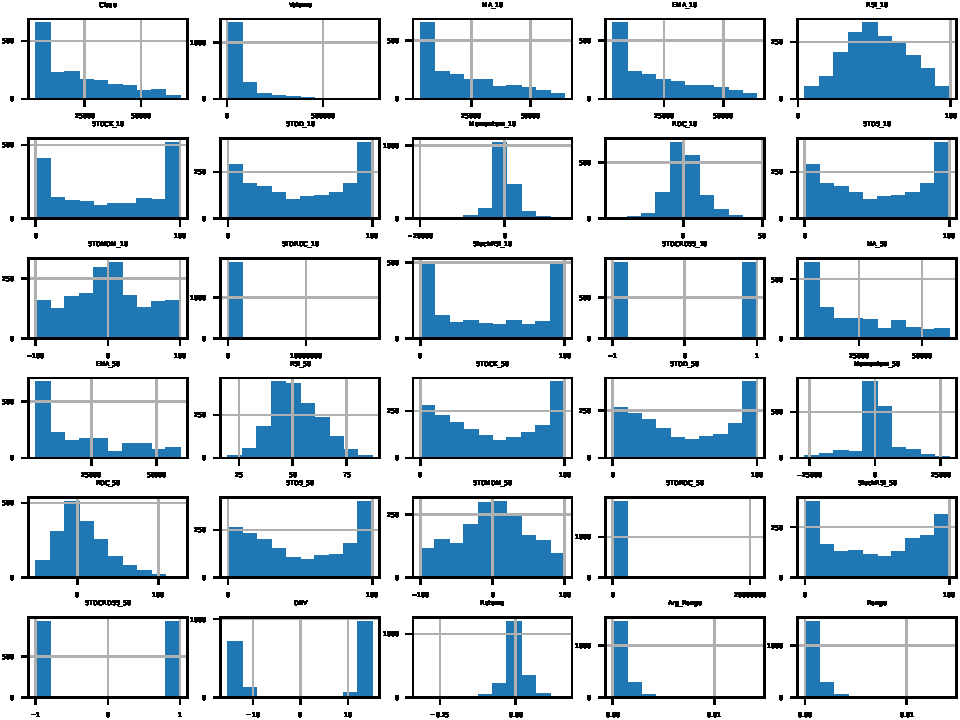
\includegraphics[page=1, trim=0 0 0 0, width=\textwidth, clip]{./uml/dataset_histogram.pdf}
\caption{Histogram of engineered features from the BTCUSDT historical data.}
\label{fig:dataset_histogram}
\end{figure}


\begin{figure}[h]
\centering
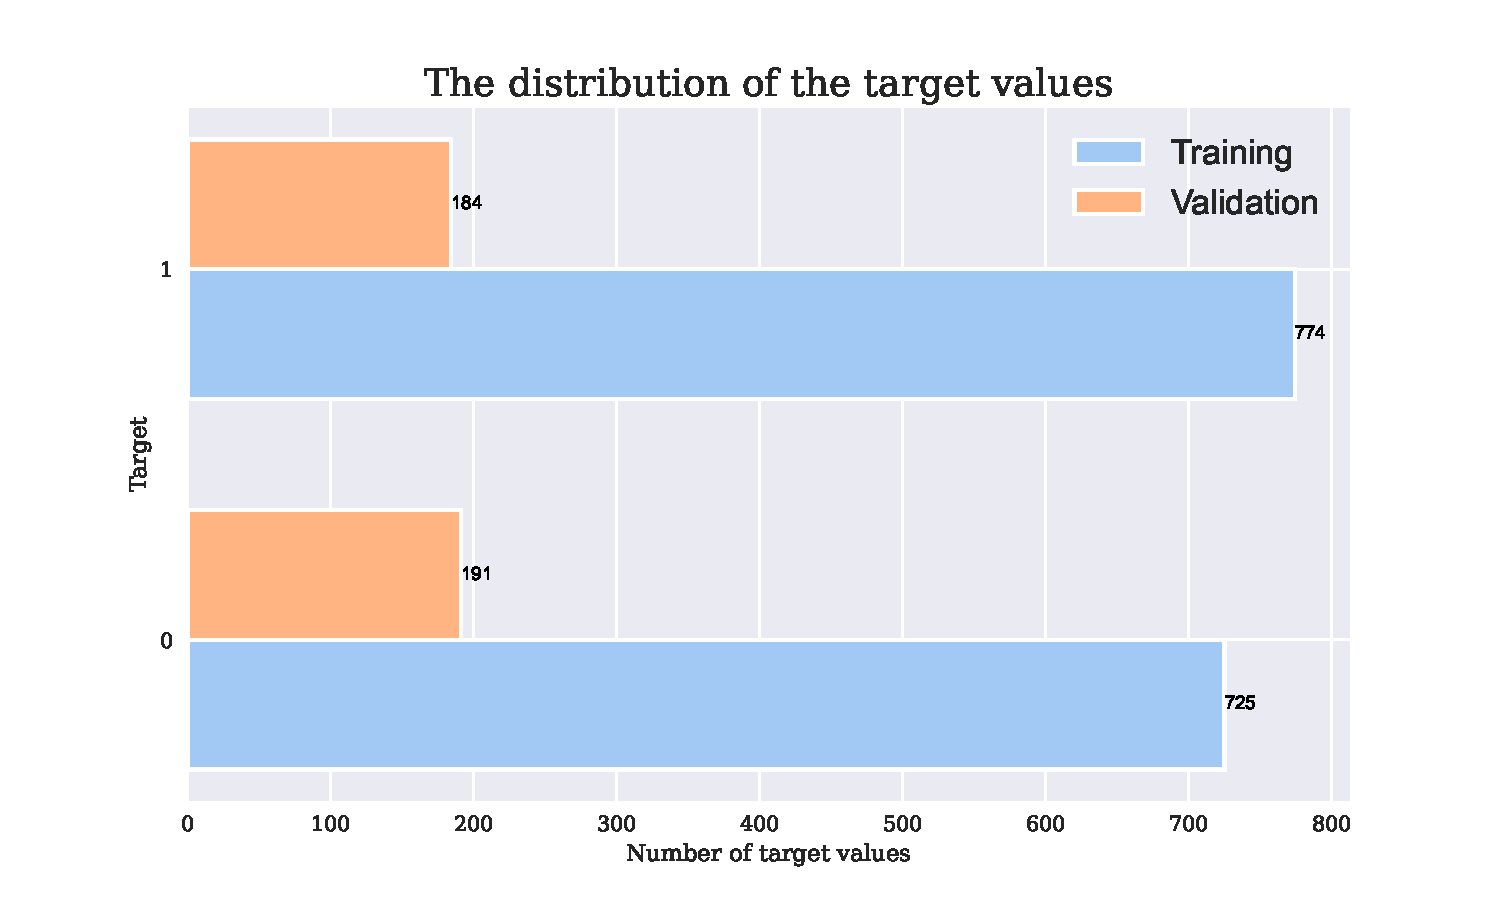
\includegraphics[width=\linewidth]{./uml/signal_distribution.pdf}
    \caption{The distribution of target values in both the training (shown in green) and validation (shown in blue) datasets. Each horizontal bar represents a unique target value, with the length of the bar indicating the count of occurrences in the respective dataset. Absolute counts are annotated directly on the bars, facilitating a clearer understanding of the distribution. This visualization aids in discerning the balance or imbalance of target values across the two datasets.}
\label{fig:signal_distribution}
\end{figure}


\begin{figure}[htbp!]
\centering
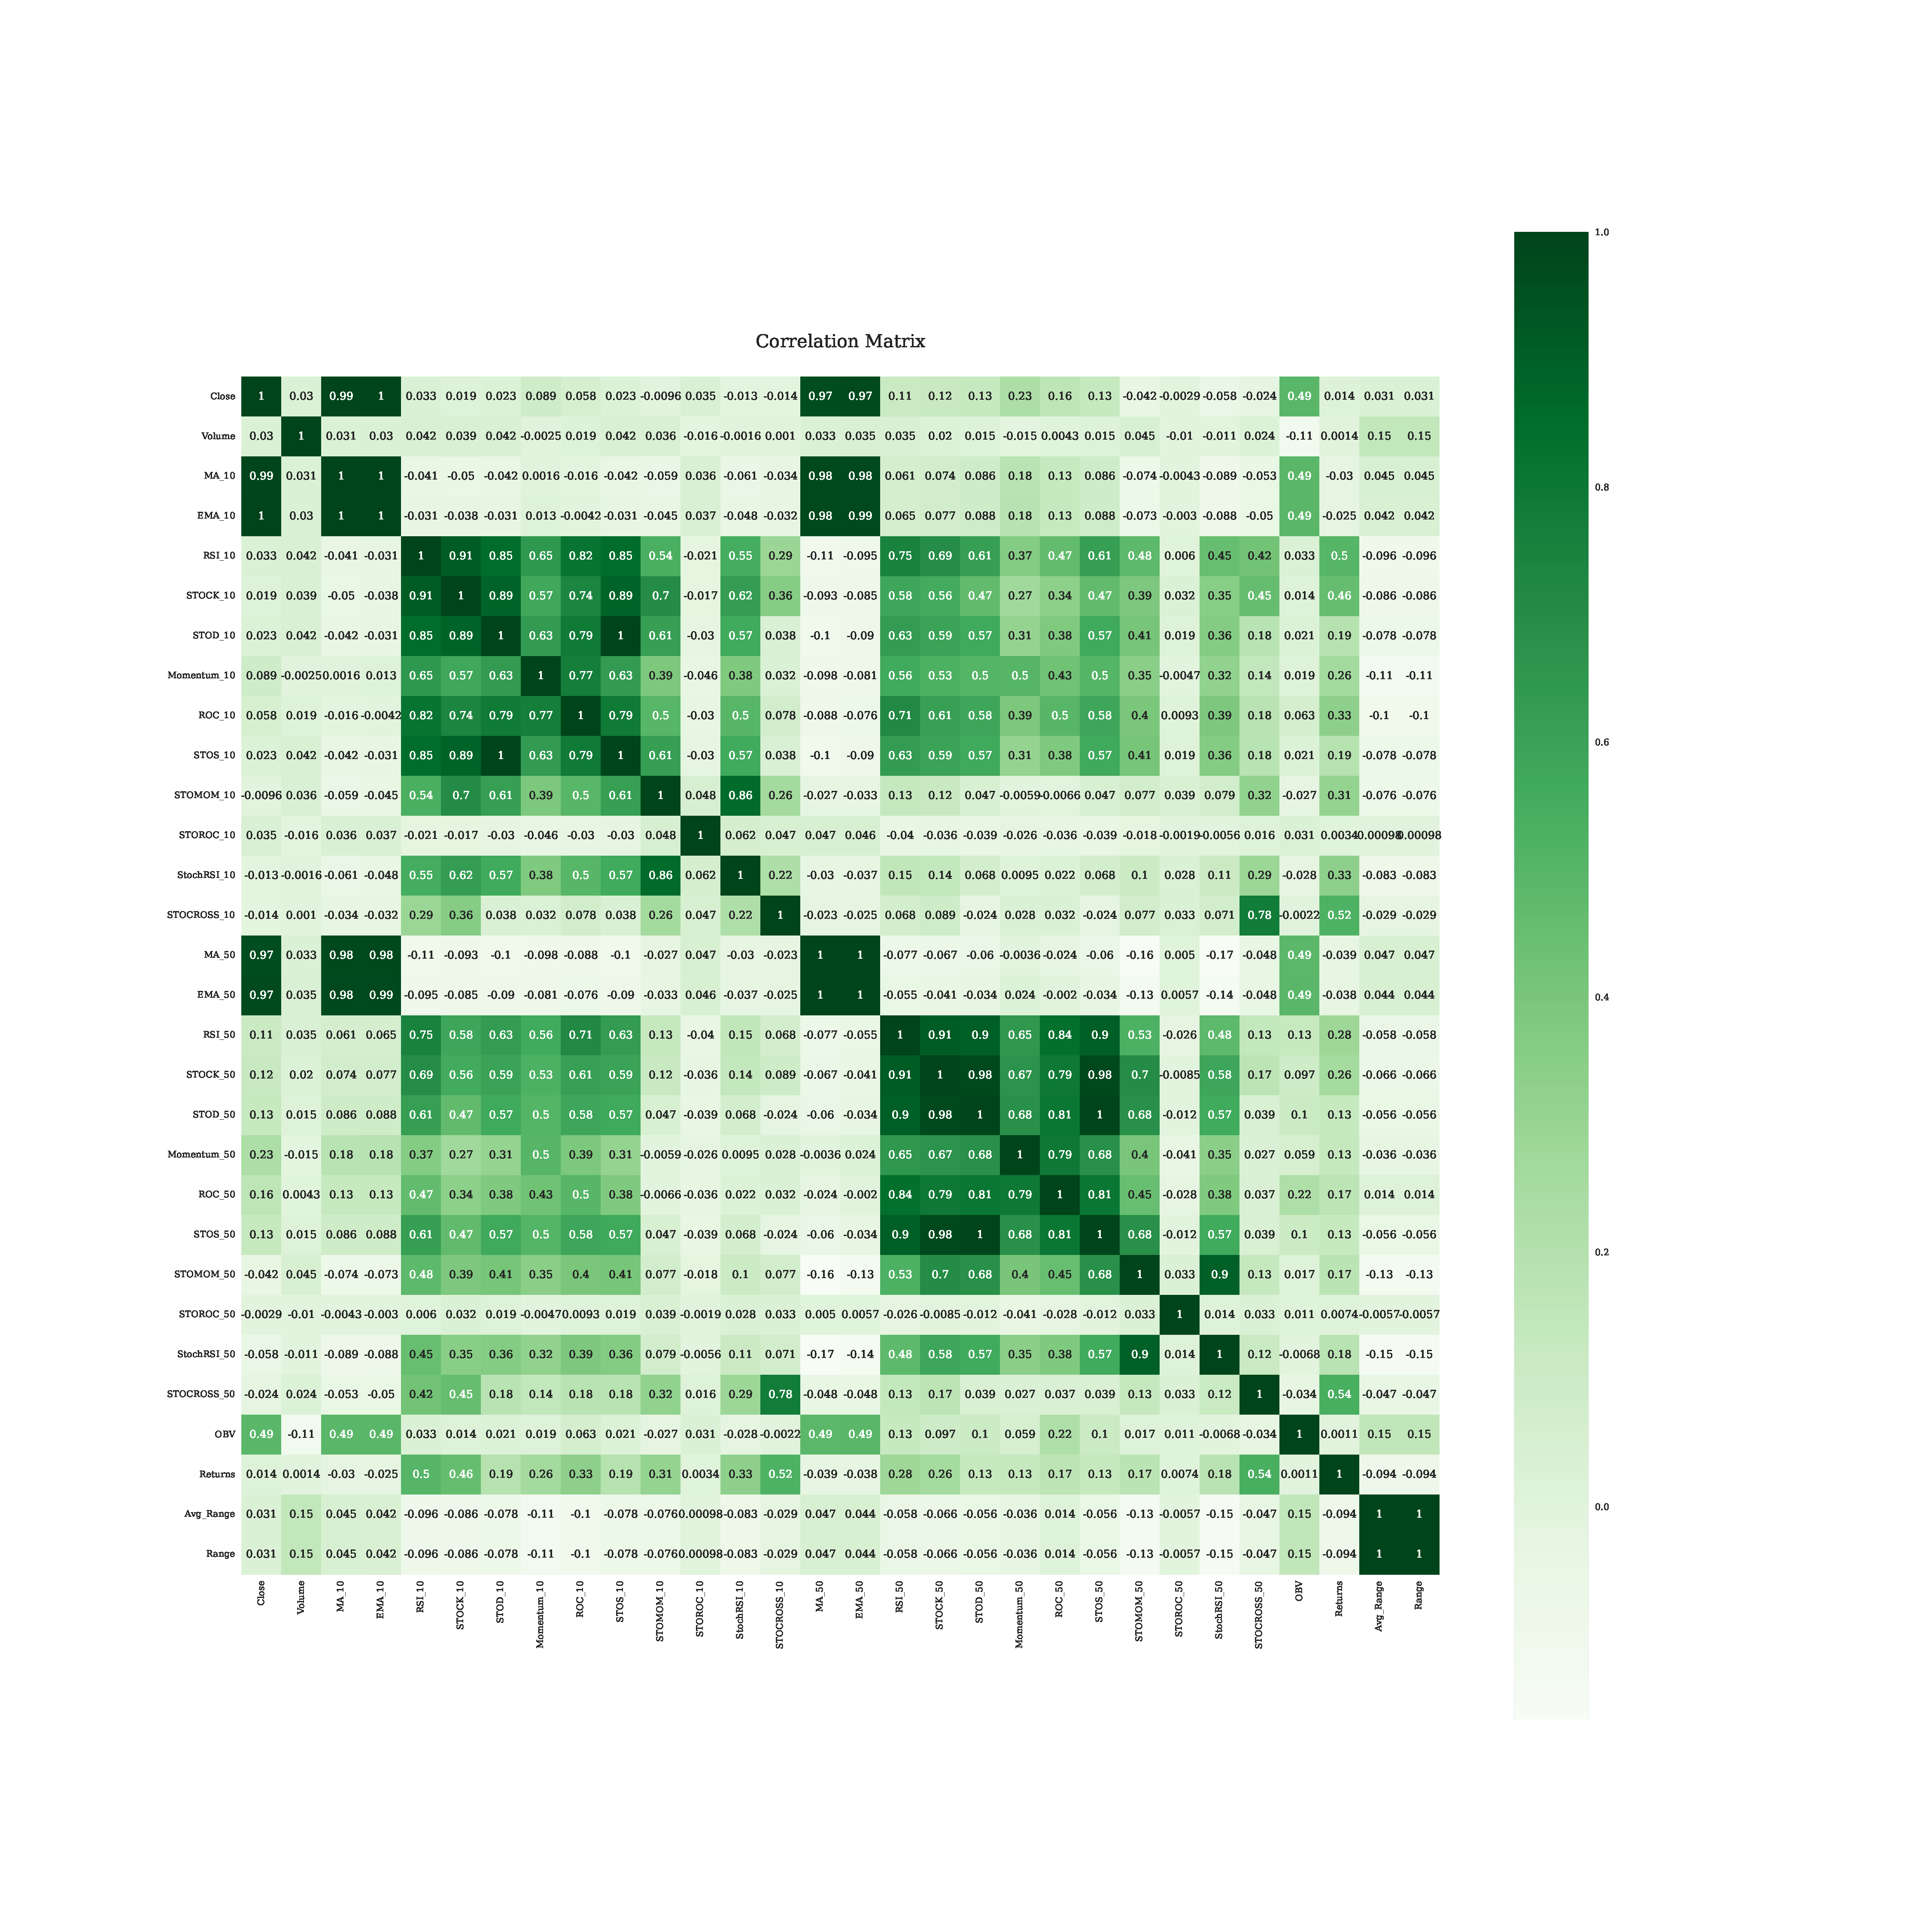
\includegraphics[width=\paperwidth]{./uml/correlation_matrix.pdf}

\caption{Correlation Coefficient between features variables.}
\label{fig:corr_coef}
\end{figure}


\section{Pipeline}

\subsection{Data Ingestion}
The initial step involves ingesting data required for backtesting. This data can either be procured using the \texttt{data\_retrieve.py} module (refer to Chapter~\ref{chap:dataRetrieve}) or loaded from the \texttt{historical\_data} folder, found within the respective symbol's subfolder. If the data hasn't been previously downloaded, it can be found here. It's recommended to retrieve data with a one-minute time bar length, as this can be efficiently downsampled later for larger intervals such as an hour or a day.

\subsection{Data Preprocessing}
In this phase, the ingested data is downsampled based on the bar length stipulated in the configuration. Furthermore, a validation check is run to ensure data integrity.

\subsection{Feature Engineering}
This step mainly focuses on constructing features derived from various technical indicators and statistical methodologies. These features could be momentum-based, volume-based, among others. Following this, a target is computed, which can also be specified in the configuration file. The available target variants include:
\begin{itemize}
    \item \textbf{Simple}: Predicts if the next day's price will go up or down based on today's closing price.
    \item \textbf{MA\_Relative}: Checks if today's closing price is above its short-term average and rising.
    \item \textbf{Momentum}: Examines if the stock's momentum is positive and increasing.
    \item \textbf{ROC}: Looks at if the rate of change (ROC) is positive and on the rise.
    \item \textbf{Consecutive\_Increases}: Predicts if returns will rise for the third consecutive time after a decline.
\end{itemize}


\begin{figure}[h]
\centering
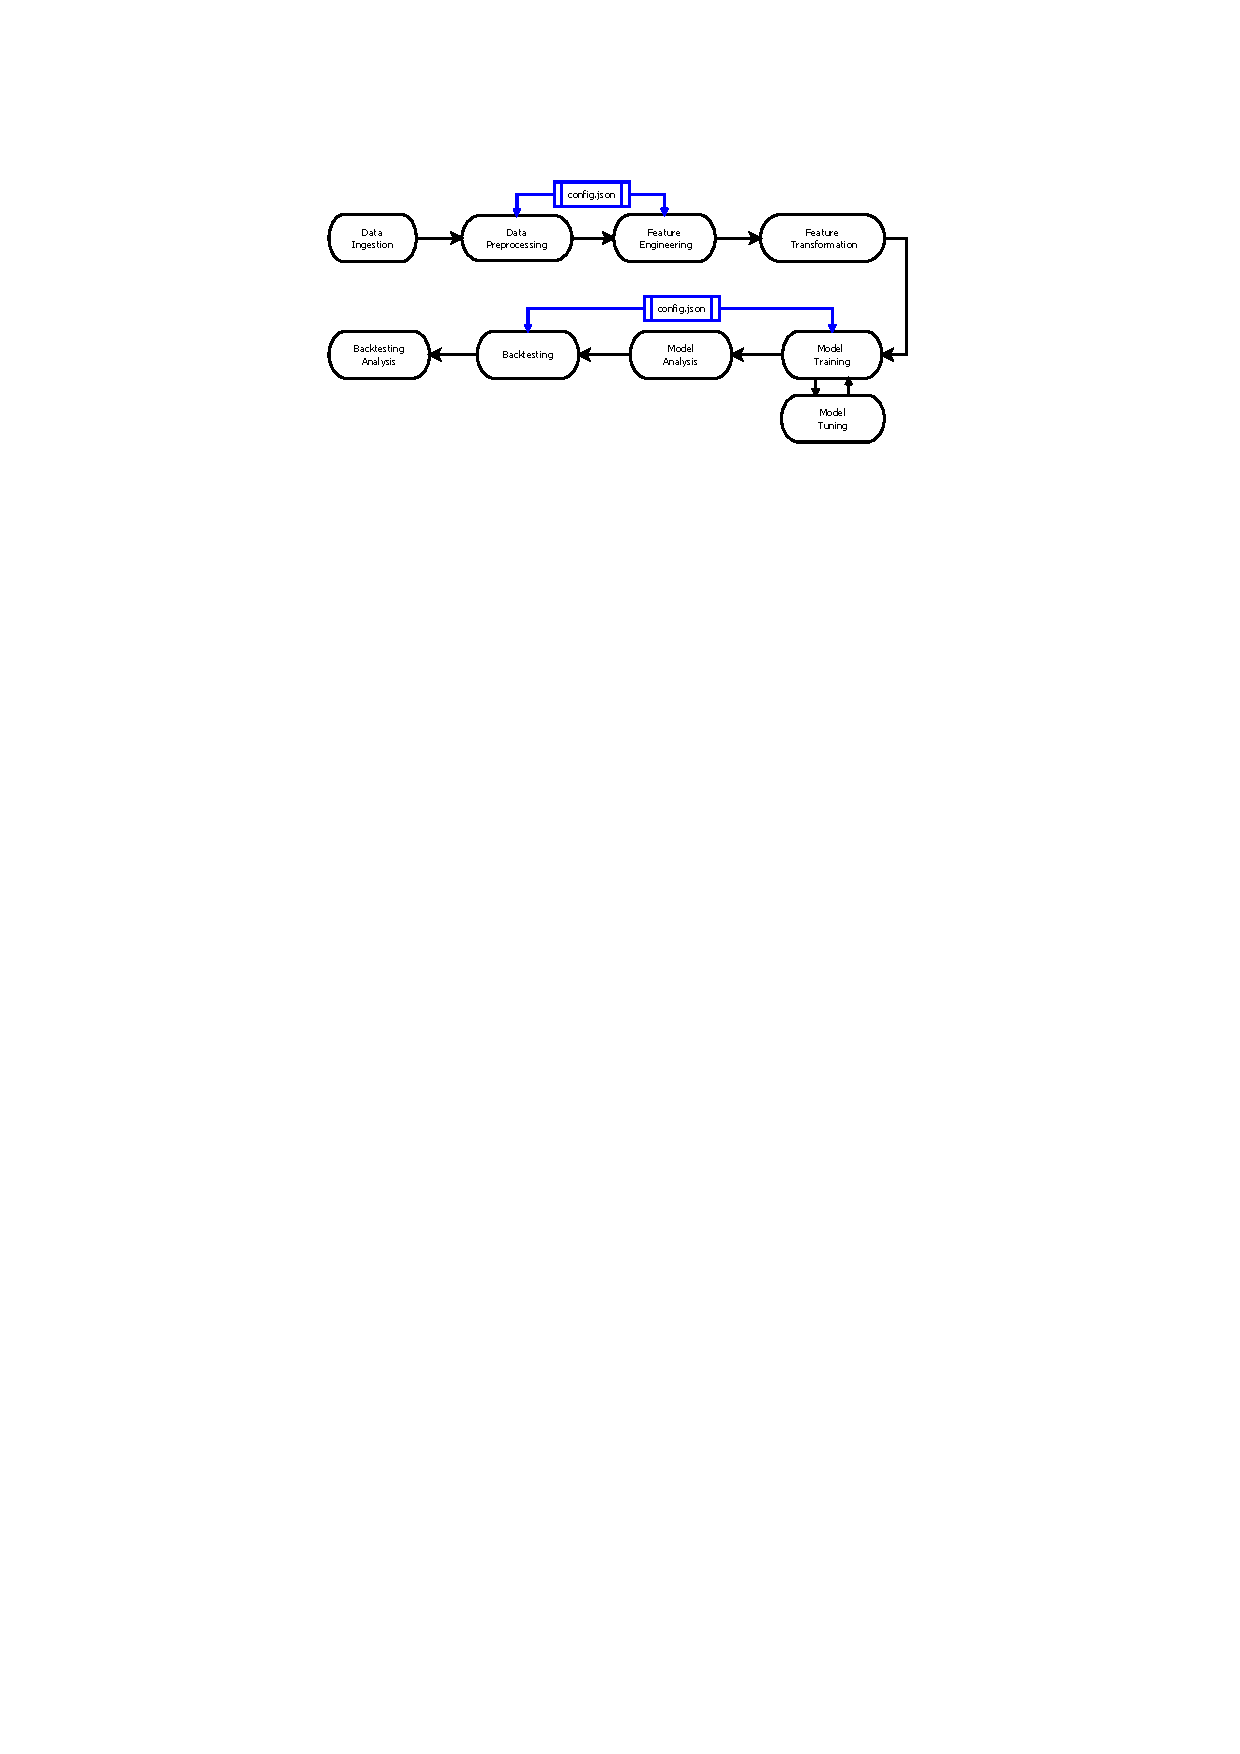
\includegraphics[page=1, trim=50mm 220mm 20mm 25mm, width=1.3\textwidth, clip]{./uml/ml_pipeline.pdf}
\caption{Technical indicator based backtesting architecture.}
\label{fig:ml_pipeline}
\end{figure}


\begin{figure}
\centering
\includegraphics[width=1.0\textwidth]{./uml/perf\_metrics.pdf}
\caption{Visualization of the Classification Report.}
\label{fig:conf_matrix}
\end{figure}

 %Confusion matrix (left) presenting actual versus predicted values, alongside key performance metrics (right) indicating the model's accuracy, precision, recall, and F1 score.}
\subsection{Feature Transformation}

Once features have been engineered, it's essential to transform them to ensure they are adjusted to meet the requirements and sensitivities of machine learning models. Different models have varied preferences when it comes to the scale and distribution of input data. This transformation process uses several techniques such as Standardization and MinMaxScaling.

It's vital to apply the same transformations, like standardization parameters, to both the training and testing datasets or any new incoming data. This ensures consistent and accurate model predictions.

The entire transformation workflow, from data loading, preprocessing, to feature-related operations, is orchestrated by the \texttt{DataManager} and \texttt{FeatureEngineer} classes (fig. \ref{fig:dataManagerFeatureEngineer}).
After this step the \texttt{ml\_model\_evaluator} module can be used for data analysis. It provides tools for both data and model checks. The prepared data can be visualized in various ways, including target distributions, feature covariance matrices, and feature histograms.


\subsection{Model Training and Optimization}
Model specifics, including the model type (e.g., LogisticRegressor) and its hyperparameter ranges, are detailed in the JSON configuration file. The optimization uses Grid Search combined with Cross-Validation, the details of which (e.g., number of folds) can also be adjusted in the configuration file (see fig. ~\ref{fig:modelConfig}).

\subsection{Model Evaluation}
After training and optimization, the model's performance is assessed using various evaluation metrics, including graphical representations like the confusion matrix. Moreover, additional plots are available to facilitate data analysis, such as the covariance matrix.

\subsection{Backtesting}
Backtesting is done in a separate step because it has its unique methods and processes. The trained and adjusted model is tested to see the returns, showing how it might have worked in real-life situations.
\subsection{Backtest Analysis}
The last step in the evaluation of backtesting results. Performance metrics in this analysis include strategy returns, comparison to a benchmark like the buy-and-hold strategy, and the usage of other advanced metrics such as Calmar and Sortino ratios.

\begin{figure}
\centering
\includegraphics[width=1.0\textwidth]{./uml/feature\_importance.pdf}
\caption{Feature Significance in Model Prediction}
\label{fig:feature_importance}
\end{figure}
